\documentclass[graybox]{svmult}

\usepackage{mathptmx}
\usepackage{helvet}
\usepackage{courier}
\usepackage{type1cm}
\usepackage[T1]{fontenc}
\usepackage[utf8]{inputenc}
\usepackage{graphicx}
\usepackage{booktabs}
\usepackage{amsmath}
\usepackage{tikz}
\usetikzlibrary{positioning,arrows.meta}
\usepackage{url}
\usepackage[hidelinks]{hyperref}
\usepackage{cite}
\usepackage[bottom]{footmisc}
\usepackage{microtype}

\newcommand{\nGauges}{19}
\newcommand{\nGaugesAlti}{7}
\newcommand{\nGaugesCB}{6}
\newcommand{\nGaugesWSA}{6}
\newcommand{\nPeru}{13}
\newcommand{\nChile}{6}
\newcommand{\nFeatures}{27}
\newcommand{\runtimeMin}{9}
\newcommand{\nBoot}{1000}
\newcommand{\bootBlock}{30}
\newcommand{\focusTestStart}{2021-09-22}
\newcommand{\focusTestEnd}{2024-12-24}
\newcommand{\focusTrainStart}{1994-09-25}
\newcommand{\focusNTestOne}{943}
\newcommand{\focusPersNseOne}{0.902}
\newcommand{\focusBestOne}{random forest}
\newcommand{\focusBestNseOne}{0.912}
\newcommand{\focusBestKgeOne}{0.924}
\newcommand{\focusBestSkillOne}{0.054}
\newcommand{\focusBestLoOne}{$-$0.003}
\newcommand{\focusBestHiOne}{0.113}
\newcommand{\focusBestDmpOne}{0.048}
\newcommand{\focusRidgeSkillOne}{0.070}
\newcommand{\focusNTestThree}{942}
\newcommand{\focusPersNseThree}{0.693}
\newcommand{\focusBestThree}{random forest}
\newcommand{\focusBestNseThree}{0.748}
\newcommand{\focusBestKgeThree}{0.822}
\newcommand{\focusBestSkillThree}{0.094}
\newcommand{\focusBestLoThree}{$-$0.004}
\newcommand{\focusBestHiThree}{0.160}
\newcommand{\focusBestDmpThree}{0.095}
\newcommand{\focusRidgeSkillThree}{0.100}
\newcommand{\focusNTestSeven}{941}
\newcommand{\focusPersNseSeven}{0.461}
\newcommand{\focusBestSeven}{Ridge regression}
\newcommand{\focusBestNseSeven}{0.578}
\newcommand{\focusBestKgeSeven}{0.677}
\newcommand{\focusBestSkillSeven}{0.115}
\newcommand{\focusBestLoSeven}{0.028}
\newcommand{\focusBestHiSeven}{0.208}
\newcommand{\focusBestDmpSeven}{0.112}
\newcommand{\focusRidgeSkillSeven}{0.115}
\newcommand{\nPosOne}{16}
\newcommand{\nSigOne}{11}
\newcommand{\nEvalOne}{19}
\newcommand{\medSkillOne}{0.051}
\newcommand{\medPersNseOne}{0.929}
\newcommand{\medBestNseOne}{0.934}
\newcommand{\medSkillAltiOne}{0.060}
\newcommand{\medSkillCBOne}{0.033}
\newcommand{\medSkillWSAOne}{0.053}
\newcommand{\nRidgePosOne}{14}
\newcommand{\nPosThree}{17}
\newcommand{\nSigThree}{12}
\newcommand{\nEvalThree}{19}
\newcommand{\medSkillThree}{0.080}
\newcommand{\medPersNseThree}{0.765}
\newcommand{\medBestNseThree}{0.787}
\newcommand{\medSkillAltiThree}{0.062}
\newcommand{\medSkillCBThree}{0.078}
\newcommand{\medSkillWSAThree}{0.083}
\newcommand{\nRidgePosThree}{18}
\newcommand{\nPosSeven}{17}
\newcommand{\nSigSeven}{12}
\newcommand{\nEvalSeven}{19}
\newcommand{\medSkillSeven}{0.108}
\newcommand{\medPersNseSeven}{0.546}
\newcommand{\medBestNseSeven}{0.620}
\newcommand{\medSkillAltiSeven}{0.103}
\newcommand{\medSkillCBSeven}{0.097}
\newcommand{\medSkillWSASeven}{0.130}
\newcommand{\nRidgePosSeven}{18}
\newcommand{\mostSelected}{Ridge regression}
\newcommand{\mostSelectedN}{11}
\newcommand{\pctDeltaTarget}{66}
\newcommand{\medCsiPers}{0.43}
\newcommand{\medCsiBest}{0.25}
\newcommand{\medCsiXgbLog}{0.33}
\newcommand{\medFarPers}{0.39}
\newcommand{\medFarBest}{0.38}
\newcommand{\medPodPers}{0.60}
\newcommand{\medPodBest}{0.44}
\newcommand{\nCsiBestBeats}{3}
\newcommand{\nCsiXgbLogBeats}{2}
\newcommand{\medCsiCalPers}{0.45}
\newcommand{\medCsiCalBest}{0.40}
\newcommand{\medPodCalBest}{0.68}
\newcommand{\medFarCalBest}{0.53}
\newcommand{\nCsiCalBestBeats}{3}
\newcommand{\nCsiCalImproves}{11}
\newcommand{\nFusion}{7}
\newcommand{\fusionMedDeltaRidge}{$-$0.005}
\newcommand{\fusionNPosRidge}{2}
\newcommand{\fusionMedDeltaXGBoost}{$-$0.008}
\newcommand{\fusionNPosXGBoost}{2}
\newcommand{\glofasMedNse}{$-$0.10}
\newcommand{\glofasNPosNse}{1}
\newcommand{\nChirps}{13}
\newcommand{\chirpsMedDeltaRidge}{$-$0.009}
\newcommand{\chirpsNPosRidge}{4}
\newcommand{\chirpsMaxDeltaRidge}{0.004}
\newcommand{\chirpsMedDeltaXGBoost}{$-$0.013}
\newcommand{\chirpsNPosXGBoost}{6}
\newcommand{\chirpsMaxDeltaXGBoost}{0.602}
\newcommand{\eraChirpsRatio}{2.8}
\newcommand{\wfNFolds}{57}
\newcommand{\wfNPos}{53}
\newcommand{\wfMedSkill}{0.103}
\newcommand{\wfFocusSkills}{0.166, 0.116, 0.114}
\newcommand{\nPairs}{104}
\newcommand{\corrDzero}{582}
\newcommand{\corrDzeroLo}{330}
\newcommand{\corrDzeroHi}{1069}
\newcommand{\corrC}{0.35}
\newcommand{\rhoDist}{$-$0.56}
\newcommand{\pDist}{$<$0.001}
\newcommand{\rhoSameRegion}{0.28}
\newcommand{\rhoCrossRegion}{0.09}
\newcommand{\moranI}{$-$0.012}
\newcommand{\moranP}{0.540}
\newcommand{\moranExp}{$-$0.056}
\newcommand{\topDriver}{snow fraction}
\newcommand{\topDriverRho}{$-$0.45}
\newcommand{\topDriverP}{0.056}
\newcommand{\topDriverPholm}{0.394}
\newcommand{\githubUrl}{https://github.com/Andre031222/streamflow-drought-altiplano}
\newcommand{\orcidAndre}{0009-0003-2385-5263}
\newcommand{\orcidMaribel}{0009-0003-6218-2735}
\newcommand{\orcidRenato}{0009-0005-2367-7852}
\newcommand{\emailAndre}{75521963@est.unap.edu.pe}
\newcommand{\emailMaribel}{maribelbel201314@gmail.com}
\newcommand{\emailRenato}{72535253@est.unap.edu.pe}

\newcommand{\phoneAndre}{}
\InputIfFileExists{private.tex}{}{}
\newcommand{\phoneLine}{\ifx\phoneAndre\empty\else, Tel.:~\mbox{\phoneAndre}\fi}
\makeatletter
\newcommand{\inputtable}[1]{\@@input #1 }
\makeatother

\hypersetup{
  pdftitle={When Machine Learning Beats Persistence: A Leakage-Free Streamflow and Drought Benchmark for the Tropical Andes},
  pdfauthor={Richar Andre Vilca-Solorzano; Renato Quispe-Vargas; Dina Maribel Yana-Yucra},
  pdfkeywords={Tropical Andes, Altiplano, Streamflow forecasting, Hydrological drought, Machine learning, Data leakage, Benchmark}}

\begin{document}

\title*{When Machine Learning Beats Persistence: A Leakage-Free Streamflow and Drought Benchmark for the Tropical Andes}
\titlerunning{Leakage-Free Andean Streamflow--Drought Benchmark}
\author{Richar Andre Vilca-Solorzano, Renato Quispe-Vargas and Dina Maribel Yana-Yucra}
\authorrunning{R. A. Vilca-Solorzano et al.}
\maketitle

\vspace*{-26mm}
\noindent{\small Faculty of Statistical and Computer Engineering, Universidad Nacional del Altiplano, Av.~Floral 1153, Puno 21001, Peru\\[2pt]
\textbf{Corresponding author:} R.\,A. Vilca-Solorzano, \href{mailto:\emailAndre}{\emailAndre}\phoneLine\\
R. Quispe-Vargas, \href{mailto:\emailRenato}{\emailRenato}; D.\,M. Yana-Yucra, \href{mailto:\emailMaribel}{\emailMaribel}\\[2pt]
ORCID: \mbox{R.\,A.\,V.-S. \orcidAndre{}}; \mbox{R.\,Q.-V. \orcidRenato{}};\\ \mbox{D.\,M.\,Y.-Y. \orcidMaribel{}}}
\par\medskip

\abstract*{Machine-learning studies of Andean streamflow rarely compare their models with persistence, and their validation designs can leak information from the test period. We built an open benchmark of \nGauges{} long-record gauges from the Andean Glacierized Catchment dataset in three regions: the Altiplano, including Puente Isla Cabanillas in the Lake Titicaca basin, the Cordillera Blanca, and the western and southern Andes. Daily discharge was combined with ERA5, MERRA-2 and CHIRPS precipitation and GloFAS~v4 simulated discharge. Six learners were compared with persistence and climatology at 1-, 3- and 7-day leads under a calendar-continuous, embargoed protocol tuned on three validation blocks. Uncertainty was estimated with block-bootstrap intervals and Diebold--Mariano tests. The learners beat persistence at \nPosOne{} of \nGauges{} gauges at one day and at \nPosSeven{} of \nGauges{} at seven days (median skill \medSkillSeven{}). Lower error did not improve drought detection: the median critical success index of drought days was \medCsiPers{} for persistence and \medCsiBest{} for the learners. A drought threshold calibrated on validation data raised it to \medCsiCalBest{}, close to but still below persistence (\medCsiCalPers{}). Drought synchrony decayed over about \corrDzero~km.}

\abstract{Machine-learning studies of Andean streamflow rarely compare their models with persistence, and their validation designs can leak information from the test period. We built an open benchmark of \nGauges{} long-record gauges from the Andean Glacierized Catchment dataset in three regions: the Altiplano, including Puente Isla Cabanillas in the Lake Titicaca basin, the Cordillera Blanca, and the western and southern Andes. Daily discharge was combined with ERA5, MERRA-2 and CHIRPS precipitation and GloFAS~v4 simulated discharge. Six learners were compared with persistence and climatology at 1-, 3- and 7-day leads under a calendar-continuous, embargoed protocol tuned on three validation blocks. Uncertainty was estimated with block-bootstrap intervals and Diebold--Mariano tests. The learners beat persistence at \nPosOne{} of \nGauges{} gauges at one day and at \nPosSeven{} of \nGauges{} at seven days (median skill \medSkillSeven{}). Lower error did not improve drought detection: the median critical success index of drought days was \medCsiPers{} for persistence and \medCsiBest{} for the learners. A drought threshold calibrated on validation data raised it to \medCsiCalBest{}, close to but still below persistence (\medCsiCalPers{}). Drought synchrony decayed over about \corrDzero~km.
\keywords{Tropical Andes $\cdot$ Altiplano $\cdot$ Streamflow forecasting $\cdot$ Hydrological drought $\cdot$ Machine learning $\cdot$ Data leakage}}

\section{Introduction}
\label{sec:intro}

Rivers of the tropical Andes supply irrigation, hydropower and drinking water, but their flow is strongly seasonal. On the Altiplano, rivers such as the Coata--Cabanillas feed Lake Titicaca and depend on a short austral-summer wet season \cite{garreaud2003altiplano}, and hydrological droughts are projected to become longer and more frequent \cite{zubieta2021titicaca}. Short-range forecasts are therefore useful, but gauges are sparse and records gappy.

Machine learning (ML) is widely used to forecast streamflow \cite{nearing2021role}. At daily leads, however, discharge is so autocorrelated that persistence, $\hat{Q}_{t+h}=Q_t$, is hard to beat \cite{pappenberger2015benchmarks}. Reported gains can be inflated by weak references, by shuffled cross-validation that leaks temporal information \cite{bergmeir2012cv,torres2026blockedcv}, and by giving the baseline and the learners different information at the time of issue. An earlier version of our own pipeline made the last error, and gave the learners discharge only up to $t-1$.

We measured how much ML adds to persistence for 1- to 7-day streamflow and drought forecasts in the Andes when no information leaks from the test period. The paper makes four contributions: (i) an open benchmark of \nGauges{} gauges in three hydroclimatic regions; (ii) a leakage-free protocol checked by automated tests; (iii) skill against persistence with confidence intervals, compared with earlier Andean studies; and (iv) a direct, calibrated evaluation of drought-day detection. Section~\ref{sec:related} reviews related work, Sect.~\ref{sec:data} describes the data and methods, Sect.~\ref{sec:results} presents the results, Sect.~\ref{sec:discussion} discusses them with their limitations, and Sect.~\ref{sec:conclusion} concludes.

\section{Related Work}
\label{sec:related}

Data-driven runoff forecasting in the Andes includes random forests and LSTM networks for hourly flows in Ecuador \cite{munoz2018rf,contreras2021rf,merizalde2023lstm}, LSTM flood warning and random forests in Chile \cite{delafuente2019lstm,nunez2023xai}, and support-vector regression in Argentina \cite{teverovsky2023svr}. In Peru, neural networks and $k$-nearest neighbours were used in two basins, including the Ramis River on the Altiplano \cite{ramos2023crisnejas,quispe2023ramis}. Table~\ref{tab:lit} summarizes these studies. Seven of the eight used a single target gauge, none compared the models with persistence, and none reported an uncertainty estimate for the skill. For Peruvian agricultural data, blocked cross-validation showed that random folds overstate accuracy \cite{torres2026blockedcv}. Drought forecasts also need an explicit identification step \cite{sutanto2021definitions}, so we score drought days directly.

\begin{table}[tb]
\centering
\caption{Data-driven streamflow studies in the Andes. Pers.: persistence reference; CI: uncertainty of skill. Scores as reported by the authors.}
\label{tab:lit}
\scriptsize
\setlength{\tabcolsep}{2pt}
\begin{tabular}{lllllccl}
\toprule
Study & Region & Gauges & Step, lead & Method & Pers. & CI & Reported score \\
\midrule
Mu\~noz et al.\ 2018 \cite{munoz2018rf} & Ecuador & 1 & 4--24 h & RF & no & no & NSE 0.76--0.38 \\
Contreras et al.\ 2021 \cite{contreras2021rf} & Ecuador & 1 & 4--24 h & RF & no & no & $R^2$ 0.69--0.29 \\
Merizalde et al.\ 2023 \cite{merizalde2023lstm} & Ecuador & 1 & 1--11 h & LSTM & no & no & NSE 0.93--0.67 \\
de la Fuente et al.\ 2019 \cite{delafuente2019lstm} & Chile & 9 & hourly, 3 d & LSTM & no & no & NSE $\approx$0.93--0.99 \\
N\'u\~nez et al.\ 2023 \cite{nunez2023xai} & Chile & 1 & 1--4 months & RF & no & no & $R^2$ 0.85--0.73 \\
Teverovsky et al.\ 2023 \cite{teverovsky2023svr} & Argentina & 1 & 1 month & SVR & no$^a$ & no & NSE up to 0.90 \\
V\'asquez-R.\ et al.\ 2023 \cite{ramos2023crisnejas} & Peru & 1 & monthly & ANN & no & no & $r^2$ 0.81 \\
Lujano et al.\ 2023 \cite{quispe2023ramis} & Peru (Altiplano) & 1 & 1 day & $k$-NN & no & no & NSE 0.979 \\
\midrule
This study & Peru, Chile & \nGauges{} & 1--7 days & 6 learners & yes & yes & skill \medSkillSeven{} at 7 days \\
\bottomrule
\end{tabular}

\smallskip
{\scriptsize $^a$Compared with seasonal ARIMA.}
\end{table}

\section{Data and Methods}
\label{sec:data}

\begin{figure}[tb]
\centering
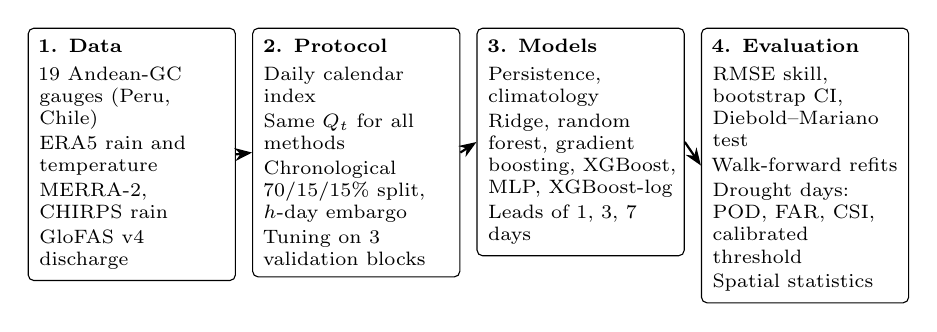
\begin{tikzpicture}[
  box/.style={draw, rounded corners=2pt, align=flush left, font=\scriptsize, text width=2.35cm, minimum height=2.7cm, inner sep=4pt, anchor=north west},
  arr/.style={-{Stealth[length=2.2mm]}, thick}]
\node[box] (d) at (0,0) {{\bfseries 1. Data}\\[2pt]
  \nGauges{} Andean-GC gauges (Peru, Chile)\\[1pt]
  ERA5 rain and temperature\\[1pt]
  MERRA-2, CHIRPS rain\\[1pt]
  GloFAS~v4 discharge};
\node[box] (p) at (2.85,0) {{\bfseries 2. Protocol}\\[2pt]
  Daily calendar index\\[1pt]
  Same $Q_t$ for all methods\\[1pt]
  Chronological 70/15/15\% split, $h$-day embargo\\[1pt]
  Tuning on 3 validation blocks};
\node[box] (m) at (5.7,0) {{\bfseries 3. Models}\\[2pt]
  Persistence, climatology\\[1pt]
  Ridge, random forest, gradient boosting, XGBoost, MLP, XGBoost-log\\[1pt]
  Leads of 1, 3, 7 days};
\node[box] (e) at (8.55,0) {{\bfseries 4. Evaluation}\\[2pt]
  RMSE skill, bootstrap CI, Diebold--Mariano test\\[1pt]
  Walk-forward refits\\[1pt]
  Drought days: POD, FAR, CSI, calibrated threshold\\[1pt]
  Spatial statistics};
\draw[arr] (d.east) -- (p.west);
\draw[arr] (p.east) -- (m.west);
\draw[arr] (m.east) -- (e.west);
\end{tikzpicture}
\caption{Workflow of the benchmark. Code, tests and result tables are in the public repository.}
\label{fig:flow}
\end{figure}

\textbf{Data.} Figure~\ref{fig:flow} summarizes the workflow. We used quality-controlled (QC) daily discharge from the Andean-GC dataset \cite{aguayo2026andeangc}. We kept every Peruvian gauge of the National Meteorological and Hydrological Service (SENAMHI) and every Chilean Altiplano gauge of the General Directorate of Water (DGA) with at least 5000 QC days. This gave \nGauges{} gauges: \nGaugesAlti{} on the Altiplano, \nGaugesCB{} in the glacier-fed Cordillera Blanca, and \nGaugesWSA{} in the western and southern Andes (Fig.~\ref{fig:map}). The focus gauge was Puente Isla Cabanillas (2843~km$^2$, mean elevation 4471~m), which drains into Lake Titicaca. Daily precipitation and 2-m temperature came from ERA5 \cite{hersbach2020era5} at each catchment centroid through Open-Meteo \cite{openmeteo}. MERRA-2 precipitation and GloFAS~v4 discharge were added in a data-fusion test, and CHIRPS v2.0 precipitation (0.05$^\circ$, averaged over each catchment, from 1981) \cite{funk2015chirps} in a resolution test at the \nChirps{} gauges with records after 1981.

\begin{figure}[tb]
\sidecaption
\includegraphics[width=0.48\textwidth]{figuras/fig00_station_map.pdf}
\caption{The \nGauges{} gauges and their catchments by region. The focus gauge, Puente Isla Cabanillas, is highlighted.}
\label{fig:map}
\end{figure}

\textbf{Forecasts and learners.} A forecast issued on day $t$ predicts $Q_{t+h}$, $h\in\{1,3,7\}$ days, from \nFeatures{} predictors available at $t$. These were discharge lags (0 to 30 days), 7- to 30-day rolling means and standard deviations, precipitation lags and 7- to 90-day totals, temperature means, and the day of year. A lag of $k$ days is exactly $k$ calendar days, and samples touching a gap were dropped. The references were persistence (same $Q_t$) and a day-of-year climatology. The six learners were Ridge regression, random forest, histogram gradient boosting, XGBoost, a two-layer perceptron (MLP), and an XGBoost trained on the change in $\log(1+Q)$ (XGBoost-log).

\textbf{Protocol.} Each record was split chronologically into 70\% training, 15\% validation and 15\% test, with an $h$-day embargo between blocks. Hyper-parameters and the target form (level or change) were chosen on the mean root-mean-square error (RMSE) over three chronological blocks: the validation block and two earlier, equally long blocks of training. The chosen model was refit on training plus validation and scored once on test. Ridge was also run in a three-fold expanding walk-forward at every gauge. Automated tests check calendar offsets, the absence of future information and the embargo.

\textbf{Scores.} We report the Nash--Sutcliffe efficiency (NSE) and the skill $S=1-\mathrm{RMSE}_{\mathrm{model}}/\mathrm{RMSE}_{\mathrm{pers}}$. Its 95\% confidence intervals (CIs) came from a moving-block bootstrap \cite{kunsch1989block}, and equal accuracy was tested with the Diebold--Mariano (DM) test \cite{diebold1995dm}. A day was in drought when $Q$ fell below the monthly 20th percentile of the fitting period \cite{sutanto2021definitions}. Detection was scored with the probability of detection (POD), false-alarm ratio (FAR) and critical success index (CSI) \cite{schaefer1990csi}. Because RMSE-trained models are conservative near the threshold, we also calibrated the drought decision: a forecast signals drought when $\hat{Q}<k\,Q_{20}$, with $k$ from 0.80 to 1.80 in steps of 0.05 chosen to maximize CSI on the validation block. The same calibration was applied to every method, including persistence. Drought synchrony was the correlation of a nonparametric 30-day standardized streamflow index (SSI-30) \cite{farahmand2015nonparametric} between gauge pairs, fitted as $\rho(d)=c\,e^{-d/d_0}$; skill clustering was tested with Moran's $I$.

\section{Results}
\label{sec:results}

\textbf{Focus gauge.} At Cabanillas (Table~\ref{tab:focus}; test period \focusTestStart{} to \focusTestEnd{}), the validation-selected \focusBestOne{} reached NSE~$=$~\focusBestNseOne{} at one day, against \focusPersNseOne{} for persistence. This is a skill of \focusBestSkillOne{} (95\% CI \focusBestLoOne{} to \focusBestHiOne{}; DM $p$~\focusBestDmpOne{}), whereas our earlier, leaky pipeline had found a loss. At seven days, persistence fell to NSE~$=$~\focusPersNseSeven{}, and the selected \focusBestSeven{} gained \focusBestSkillSeven{} (95\% CI \focusBestLoSeven{} to \focusBestHiSeven{}); its walk-forward folds gave \wfFocusSkills{}. Ridge beat persistence at all three leads with CIs above zero.

\begin{table}[tb]
\centering
\caption{Test scores at Puente Isla Cabanillas. Skill is relative to persistence, with 95\% CI. $^\dagger$Learner selected on validation. CSI: drought-day detection at seven days.}
\label{tab:focus}
\scriptsize
\setlength{\tabcolsep}{3pt}
\begin{tabular}{lrcrcr}
\toprule
& \multicolumn{2}{c}{1-day lead} & \multicolumn{2}{c}{7-day lead} & \\
\cmidrule(lr){2-3}\cmidrule(lr){4-5}
Method & NSE & Skill [95\% CI] & NSE & Skill [95\% CI] & CSI \\
\midrule
\inputtable{tab_focus_compact.tex}
\bottomrule
\end{tabular}
\end{table}

\textbf{All gauges.} The learner beat persistence at \nPosOne{}/\nGauges{}, \nPosThree{}/\nGauges{} and \nPosSeven{}/\nGauges{} gauges at 1, 3 and 7 days, and its CI excluded zero at \nSigOne{}, \nSigThree{} and \nSigSeven{} gauges (Fig.~\ref{fig:heatmap}). The median skill grew from \medSkillOne{} to \medSkillThree{} and \medSkillSeven{}, because persistence degraded faster than the learners. Between one and seven days it rose in all three regions: from \medSkillAltiOne{} to \medSkillAltiSeven{} on the Altiplano, from \medSkillCBOne{} to \medSkillCBSeven{} in the Cordillera Blanca and from \medSkillWSAOne{} to \medSkillWSASeven{} in the western and southern Andes. Ridge, the most often selected learner, was skilful at \nRidgePosSeven{}/\nGauges{} gauges at seven days, and \wfNPos{} of \wfNFolds{} walk-forward folds had positive skill (median \wfMedSkill{}).

\begin{figure}[tb]
\centering
\includegraphics[width=0.84\textwidth]{figuras/fig03_skill_heatmap_h7.png}
\caption{Seven-day RMSE skill against persistence for every gauge and method. Boxed cells: 95\% CI above zero. Gauges are grouped by region (top to bottom: Altiplano, Cordillera Blanca, western and southern Andes).}
\label{fig:heatmap}
\end{figure}

\textbf{Drought detection.} Lower RMSE did not give better detection of drought days (Fig.~\ref{fig:drought}). At seven days, the median CSI was \medCsiPers{} for persistence and \medCsiBest{} for the learner, which beat persistence at only \nCsiBestBeats{}/\nGauges{} gauges. The learners raised fewer false alarms (median FAR \medFarBest{} vs.\ \medFarPers{}) but missed more drought days (POD \medPodBest{} vs.\ \medPodPers{}). Calibration moved the learners towards more warnings (POD \medPodCalBest{}, FAR \medFarCalBest{}) and improved their CSI at \nCsiCalImproves{} gauges, to a median of \medCsiCalBest{}. Calibrated persistence reached \medCsiCalPers{} and remained better at \the\numexpr\nGauges-\nCsiCalBestBeats\relax{} gauges.

\begin{figure}[tb]
\sidecaption
\includegraphics[width=0.5\textwidth]{figuras/fig05_drought_performance_h7.pdf}
\caption{Performance diagram \cite{roebber2009performance} of seven-day drought-day detection. Small marks: gauges; large marks: medians. Curves: CSI (labelled on the diagonal); dotted lines: frequency bias $B$. The arrow shows the effect of calibrating the drought threshold.}
\label{fig:drought}
\end{figure}

\textbf{Spatial statistics.} The SSI-30 correlation of \nPairs{} gauge pairs decreased with distance (Spearman \rhoDist{}, $p$~\pDist{}), with $d_0=\corrDzero$~km (95\% CI \corrDzeroLo--\corrDzeroHi~km), and was higher within regions than across them (median \rhoSameRegion{} vs.\ \rhoCrossRegion{}). Skill showed no spatial clustering (Moran's $I=\moranI$, $p=\moranP$), and no catchment attribute was significant after Holm correction (strongest: snow fraction, $\rho=\topDriverRho$, $p=\topDriverP$).

\section{Discussion}
\label{sec:discussion}

The protocol, not the model, changed our conclusions most: with equal information and calendar lags, a one-day loss at Cabanillas became a gain. The gains are modest (median RMSE 5--11\% lower) but consistent, and Ridge was as good as tree ensembles \cite{nearing2021role}.

Earlier Andean studies report high scores, often NSE above 0.9, but none was compared with persistence (Table~\ref{tab:lit}). At Cabanillas, persistence alone reached NSE~$=$~\focusPersNseOne{} at one day and the best learner \focusBestNseOne{}. For the Ramis River, a $k$-NN model with only the previous day's discharge reached NSE~$=$~0.965, against 0.979 for the best model \cite{quispe2023ramis}. In both rivers most of the NSE comes from persistence, so a high NSE alone does not show skill.

Models trained on squared error smooth the recession limb near the drought threshold. Calibration closed most of this gap, but persistence remained the better drought reference, so warnings should be trained and verified on the drought decision itself \cite{sutanto2021definitions}. More forcing data did not help. Adding MERRA-2 and GloFAS changed the seven-day Ridge skill by a median of \fusionMedDeltaRidge{}. CHIRPS, which is 25 times finer and \eraChirpsRatio{} times drier than ERA5 at these catchments, changed it by \chirpsMedDeltaRidge{} and improved only \chirpsNPosRidge{} of \nChirps{} gauges. At short leads, recent discharge carries information that gridded rainfall does not add.

\textbf{Limitations.} Neither ERA5 nor CHIRPS resolves single convective storms on the Altiplano \cite{garreaud2003altiplano}. The Cordillera Blanca records predate MERRA-2 and GloFAS, so the fusion test covered \nFusion{} gauges only. Three selection blocks reduce, but do not remove, the effect of non-stationarity such as glacier retreat. Predictors used observed forcing up to $t$, not weather forecasts, and Andean-GC contains no Bolivian gauges.

\section{Conclusion}
\label{sec:conclusion}

We released an open, leakage-free benchmark for 1- to 7-day streamflow and drought forecasting at \nGauges{} Andean gauges. The learners beat persistence at \nPosSeven{}/\nGauges{} gauges at seven days (median skill \medSkillSeven{}). The gains did not carry over to drought-day detection; a calibrated threshold narrowed the gap but did not close it. Future work will add drought-aware training losses, operational weather forecasts and more Altiplano gauges.

\section*{Declarations}
\noindent\textbf{Data and code availability.} Discharge: Andean-GC, doi:\href{https://doi.org/10.5281/zenodo.18035801}{10.5281/zenodo.18035801}. Code, tests, gauge list, tables and supplementary figures: {\small\url{\githubUrl}}. \textbf{Author contributions.} R.\,A.V.-S.: conception, software, analysis, writing; R.Q.-V.: validation; D.\,M.Y.-Y.: supervision. All authors approved the manuscript. \textbf{Competing interests.} None. \textbf{Use of AI.} Generative AI was used to improve the language; the authors reviewed the text and take full responsibility for it.

\bibliographystyle{spmpsci}
\bibliography{references}

\end{document}
